\section{Dataset Recording}

One of the goals of this thesis, is to arrive at 

\subsection{Recording}

SilverFit conducts test sessions in 2 separate Stages. In the first stage the exercises are done by employees in a managed test environment, where different chairs are used. In the second stage real customers, who opt into participating in those tests, are instructed by a tester on how the exercise works and then possible errors are marked down in a real life scenario. In both these areas I am planning to record the data to diversify the dataset and also to include as much real life data as possible.

The recording setup should not influence the rest of the test session, by for example negatively influencing the frame rate, since the hardware has limited resources. Therefore it is essential, that the recording has a low performance footprint and also does not influence the capture speed of the camera, that is used during the test session.

As mentioned before two different cameras are currently used by SilverFit, the Orbbec and the Kinect camera. The recorder should ensure that both cameras have the possibility to be recorded. 

\subsection{Ground Truth detection}

To arrive at a reliably usable dataset a way to calculate the ground truth has to be found. The ground truth of a data point is the true value of the result, which is compared to the result of whatever uses the dataset to evaluate its performance. There are several approaches with which a ground truth can be derived. It is essential though, that the method of retrieving the ground truth is far more robust and accurate than any model that will be tested in the foreseeable future.

We therefore arrived at the conclusion, that adding more information resources just for the ground truth detection might prove essential to arrive at a method, which is robust enough to make the dataset usable in at least most cases.

One fairly obvious obstacle arises when considering the way depth data is recorded. TODOTODO

In their Paper, A Multi-view RGB-D Approach for Human Pose Estimation in Operating Rooms,\cite{MultiSourceOperation} the authors use random forests, to execute human pose estimation using multiple RGB-D sources. They made no mention of the problem above, even though they too use infra red cameras. Therefore, we proceeded to experiment the artifacts, that might happen, if multiple infrared cameras are at play at the same time.

%TODO
We conduct experiments to evaluate multi cam infrared \cite{NoiseMetrics}
\cite{realsense_multi}
\cite{multi_azure_kin}

\begin{table}[]
\centering
\begin{tabular}{llllllll}
\multicolumn{1}{l|}{}  & A & B & C & D & E & F & \\ \hline
\multicolumn{1}{l|}{A} & + & + & + & + & + & + &  \\
\multicolumn{1}{l|}{B} & + & ? & - & ? & ? & ? &  \\
\multicolumn{1}{l|}{C} & + & - & + & ? & $\tilde{}$ & ? &  \\
\multicolumn{1}{l|}{D} & + & ? & ? & + & ? & ? &  \\
\multicolumn{1}{l|}{E} & + & ? & $\tilde{}$ & ? & ? & ? &  \\
\multicolumn{1}{l|}{F} & + & ? & ? & ? & ? & ? &  \\
                       &   &   &   &   &   &    
\end{tabular}
\caption{What cameras work with each other. (A) - RGB, (B) - Orbbec Astra, (C) - Orbbec Astra  Pro, (D) - Intel RealSense D4xx, (E) - XBox One Kinect, (F) - Azure Kinect DK. "+" - Works together, "$\tilde{}$" - Works together in different programs, "?" - Might work together, "-" - Does not work together}
\label{tab:cross_table}
\end{table}

\subsubsection{IntelReal Sense}

\begin{figure}[h]
    \centering
    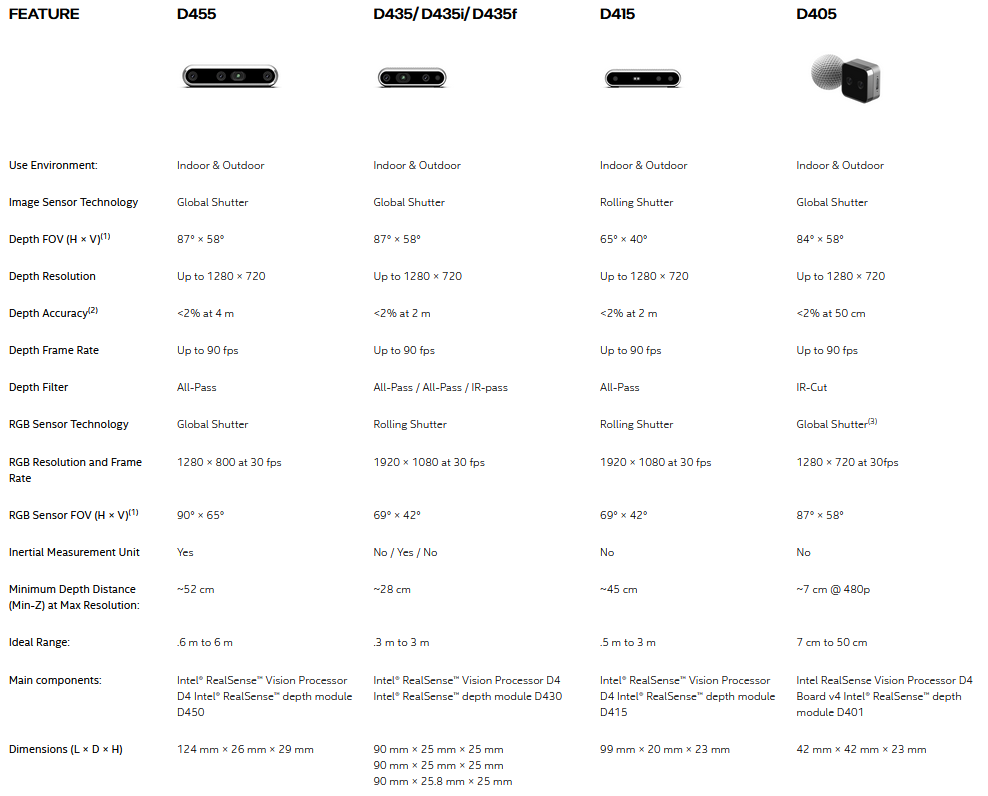
\includegraphics[width=\linewidth]{figures/IntelRealSense/IntelRealsense_cameras.png}
    \caption{Multiple Intel RealSense Cameras in comparison}
    \label{fig:realsense_cameras}
\end{figure}



\begin{figure}[h]
    \subfloat{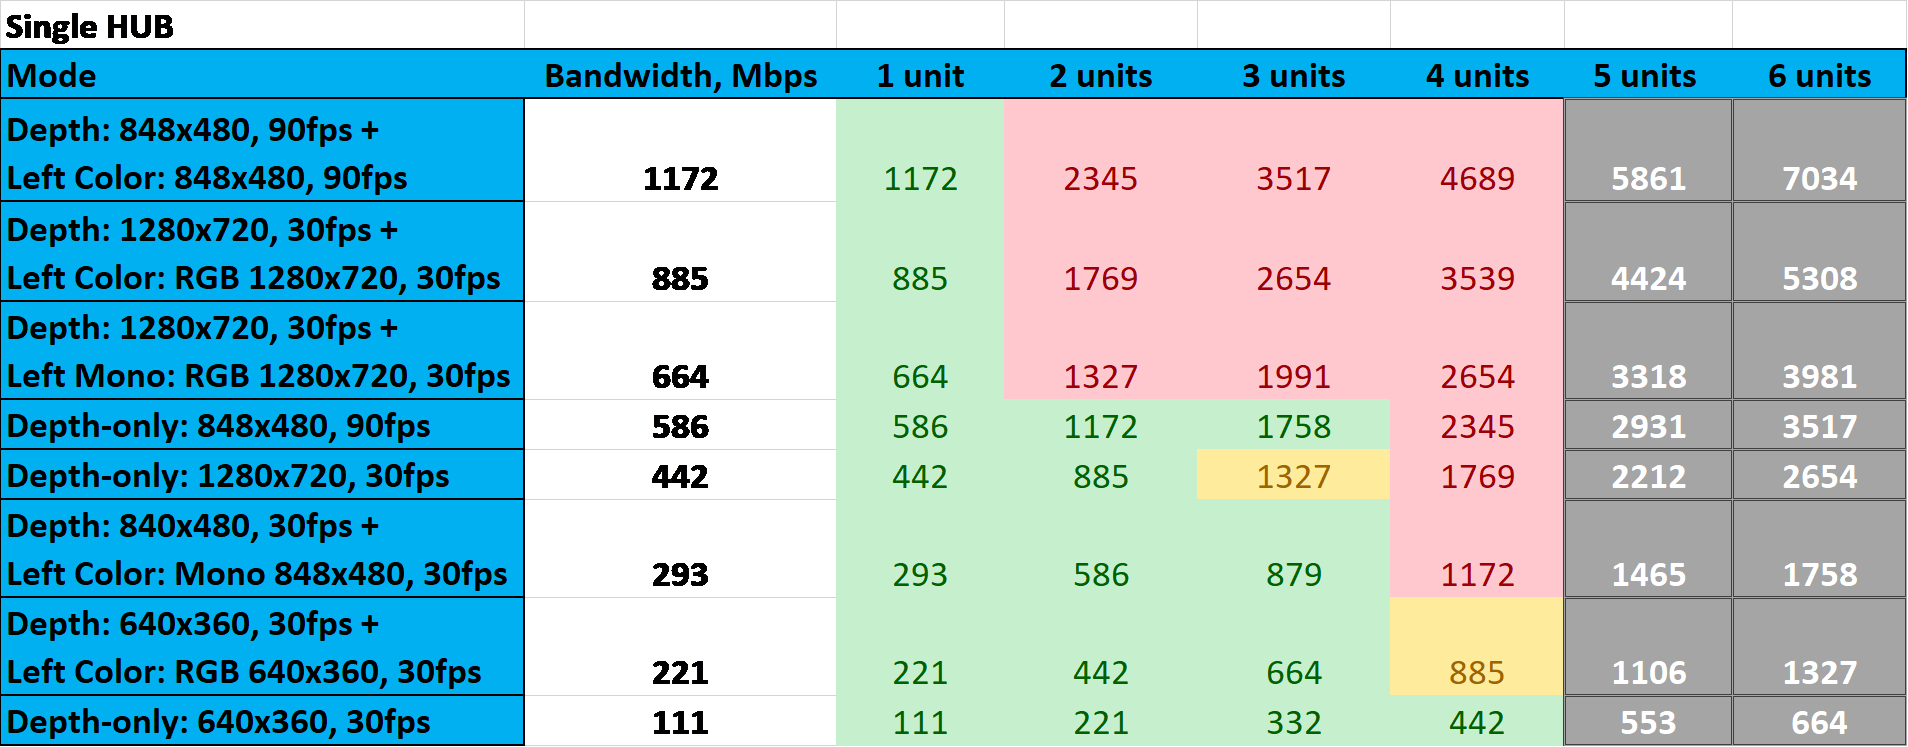
\includegraphics[width=.9\linewidth]{figures/IntelRealSense/intelRealsense_usb_hub_hw_sync.png}} \\\\
    \subfloat{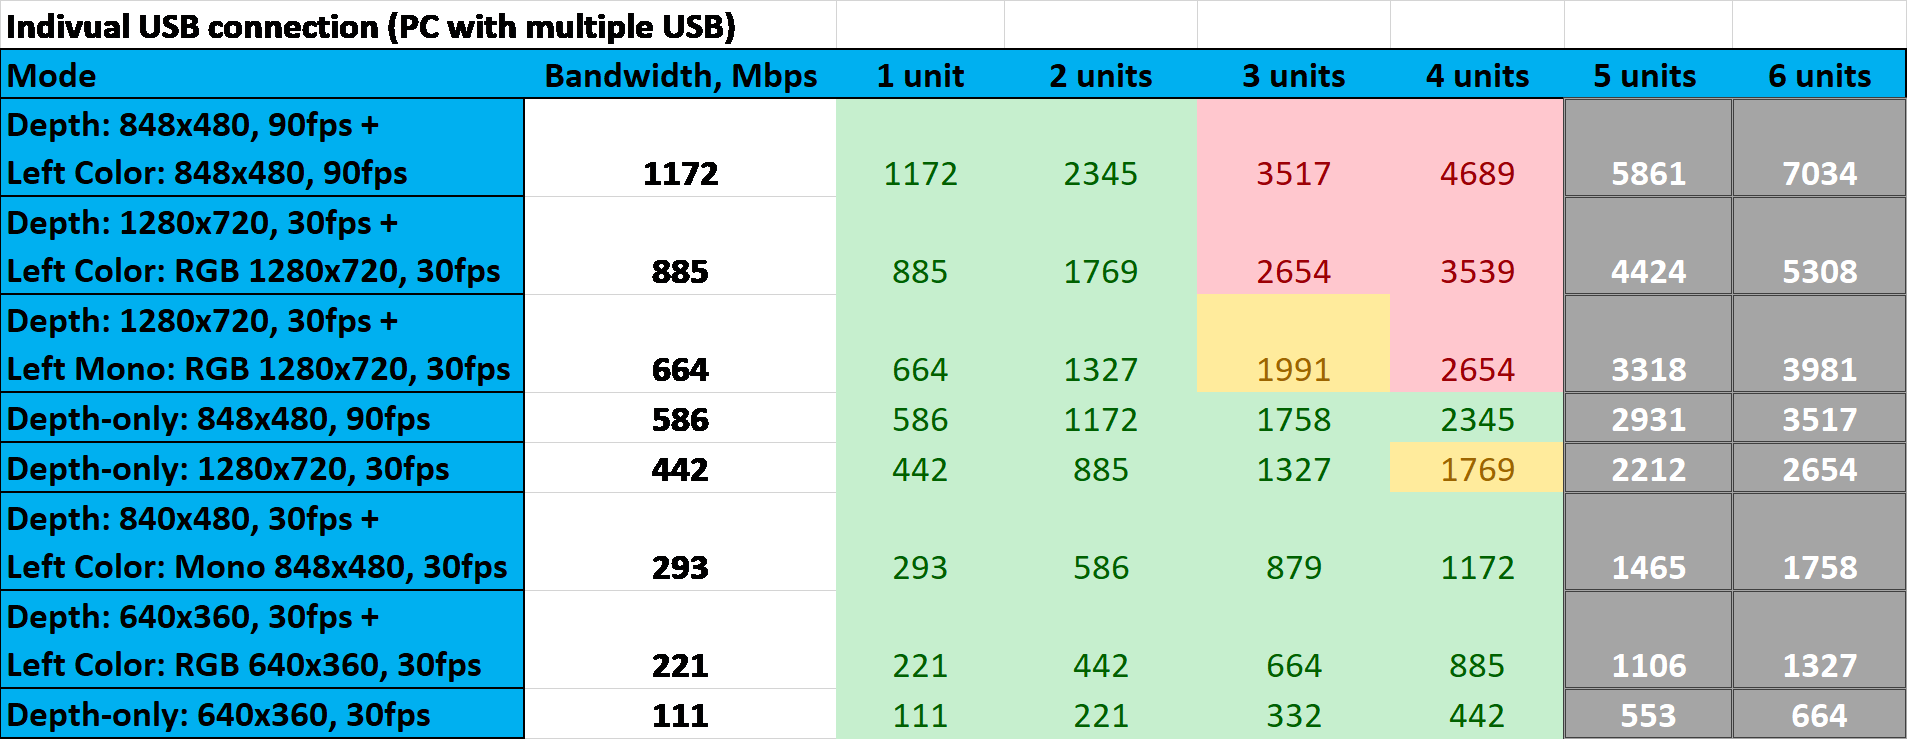
\includegraphics[width=.9\linewidth]{figures/IntelRealSense/intelRealsense_direct_hw_sync.png}} 
    \caption{Multiple Intel RealSense Cameras in comparison}
    \label{fig:hw_sync_disabled_comparison}
\end{figure}

\begin{figure}[h]
    \subfloat{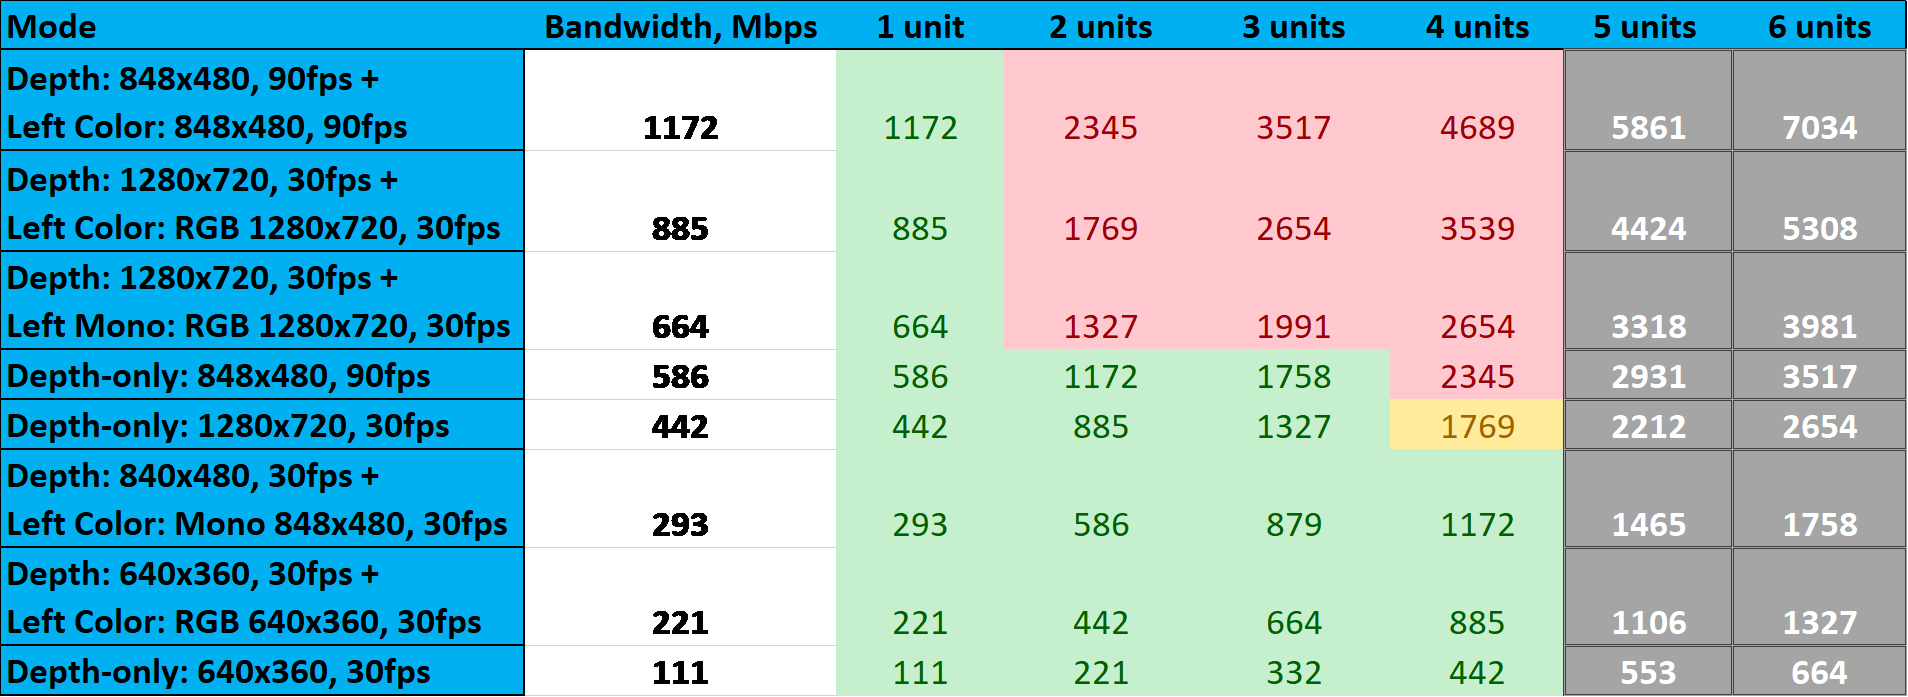
\includegraphics[width=.9\linewidth]{figures/IntelRealSense/intelRealsense_usb_hub_hw_sync_disabled.png}} \\\\
    \subfloat{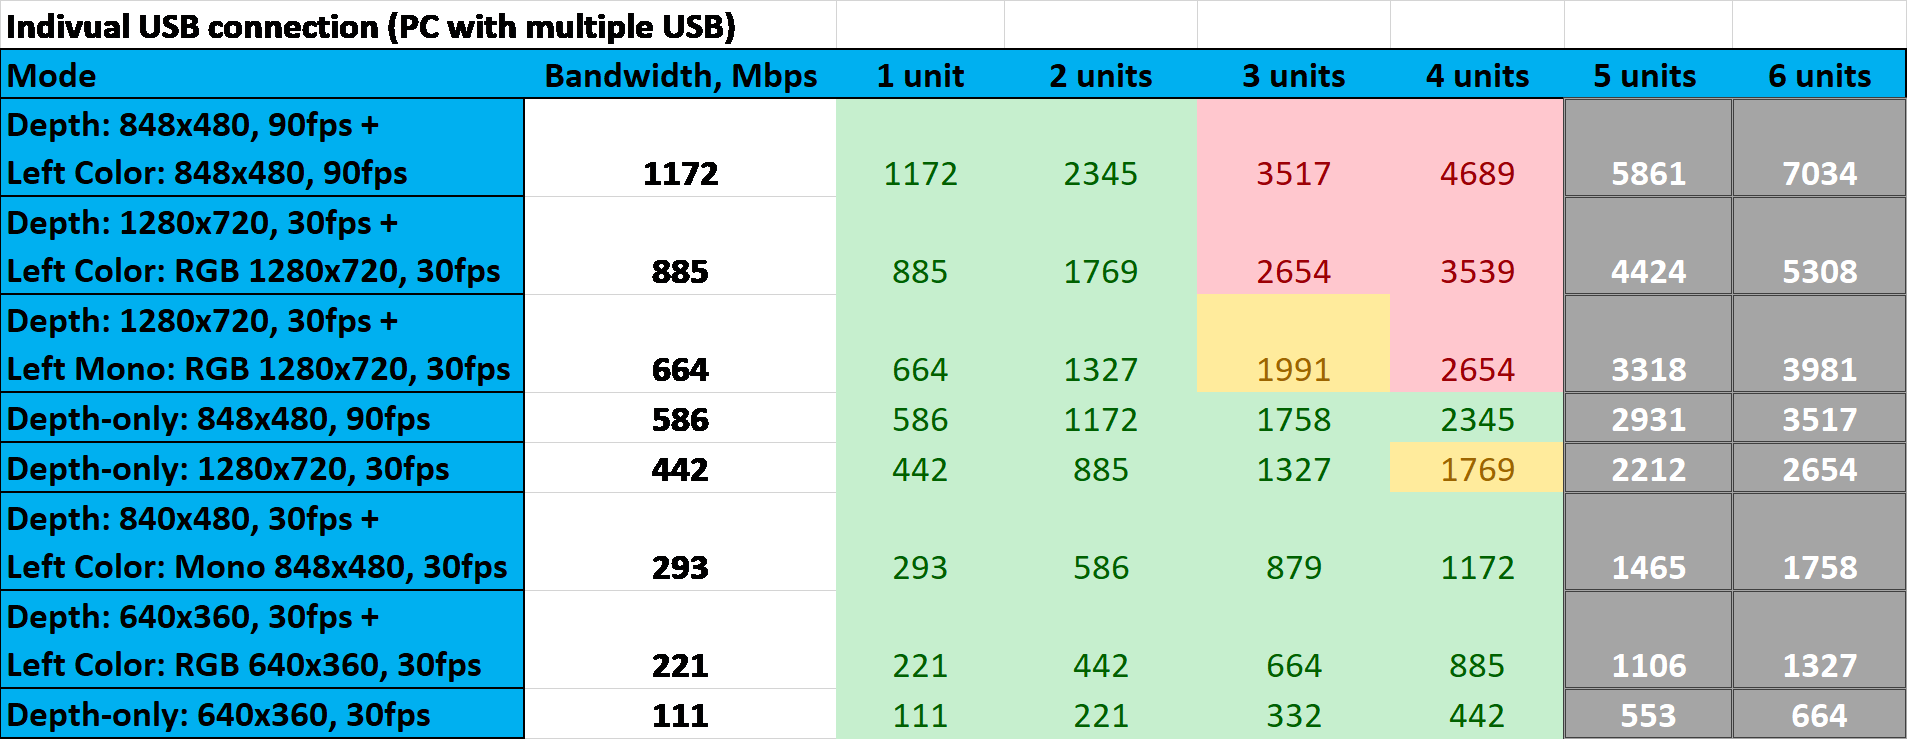
\includegraphics[width=.9\linewidth]{figures/IntelRealSense/intelRealsense_direct_hw_sync_disabled.png}} 
    \caption{Multiple Intel RealSense Cameras in comparison}
    \label{fig:hw_sync_disabled_comparison}
\end{figure}


\iffalse

\subsubsection{Monocular Depth Estimation}

In this section we will introduce the different predictors that have been examined in the scope of this project. All selected predictors are state of the art methods which have only recently been developed. Both selected methods are part of the top five for both the KITTI dataset as well as the NYU dataset, the most commonly used datasets for monocular depth estimation, we will focus on the datasets and the comparison metrics more in a later section.

Additionally to the selected algorithms others were regarded, but later discarded due to difficulties in the implementation. These also seemed to be quite promising but alas this was not within the scope of this project.

The plan was to utilise the very promising Monocular-Depth-Estimation Toolbox which was introduced by Zhenyu et.al. in \cite{toolbox}. A multitude of algorithms are available for comparison, including Depthformer \cite{mono_depthestimation_depthformer}, which introduced the toolbox and BinsFormer \cite{mono_depthestimation_binsformer} which was also introduced by Zhenyu et.al, both of which are included in the top three based on the results of on the KITTI dataset and the NYU dataset as can be seen on \cite{paperswithcode}.

\paragraph{GLPN: Global-Local Path Networks for Monocular Depth Estimation with Vertical CutDepth}

The first estimator we focus on is Global-Local Path Networks (GLPN) \cite{mono_depthestimation_glpn} which was introduced by Kin et.al. in 2022. It extracts global and local features and creates paths which are passed into various layers of CNNs.

To increase the size of the training dataset a data augmentation for depth images is applied, CutDepth \cite{cutdepth}. In CutDepth part of the depth image is cut into the training image, as can be seen in Figure \ref{fig:cutdepth}.

\begin{figure}
    \centering
    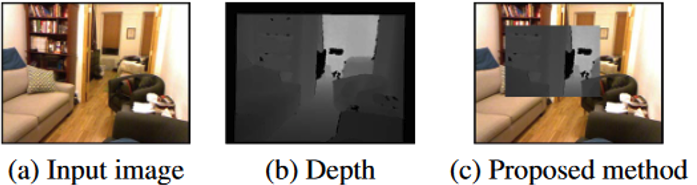
\includegraphics[width=.8\linewidth]{figures/Monocular_depth/cutdepth.png}
    \caption{An example for Cutdepth applied on training data}
    \label{fig:cutdepth}
\end{figure}

Like a lot of depth estimators, this one is also heavily influenced by Big to Small: Multi-Scale Local Planar Guidance for Monocular Depth Estimation \cite{bts}.

The architecture of the network can be seen in Figure \ref{fig:glpn}. First the global and local features are extracted and paths are formed, then various levels of CNNs are applied until finally a sigmoid funtion is applied to extract the Depth Map.

\begin{figure}
    \centering
    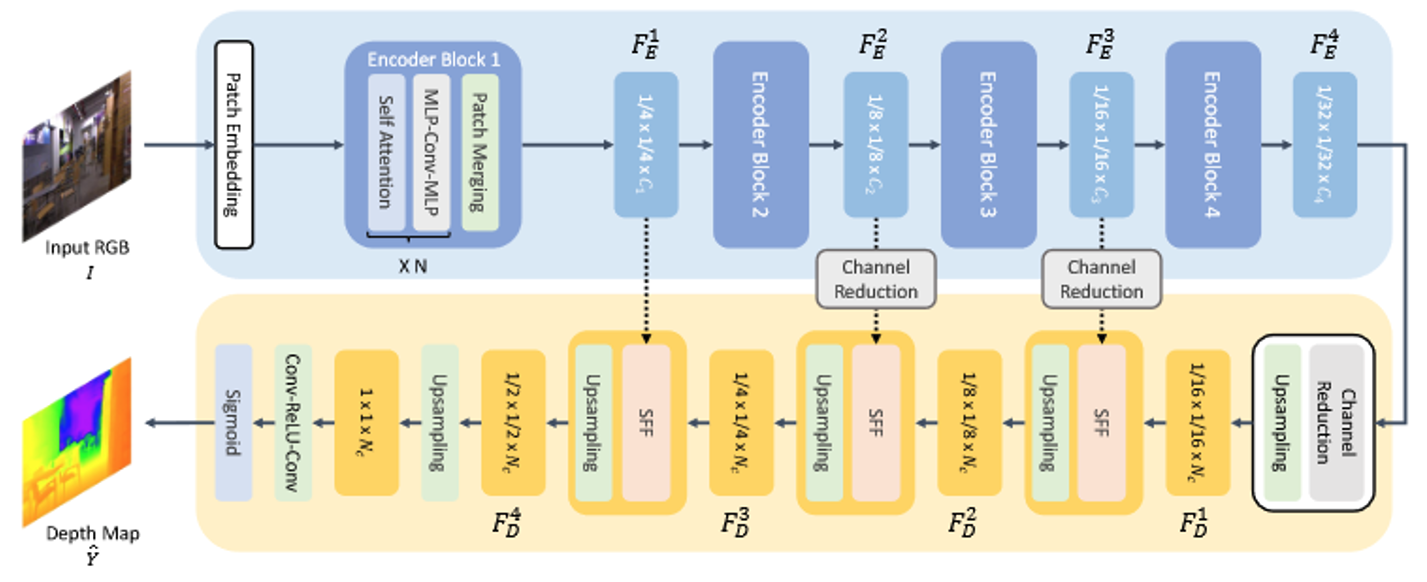
\includegraphics[width=\linewidth]{figures/Monocular_depth/glpn.png}
    \caption{The general architecture of a GLPN.}
    \label{fig:glpn}
\end{figure}


\paragraph{NeWCRFs: Neural Window Fully-connected CRFs for Monocular Depth Estimation}

Secondly we chose Neural Window Fully-connected CRFs (NeWCRFs) \cite{mono_depthestimation_newcrfs} which was introduced by Yuan et.al in 2022 in. It uses Conditional Random Fields(CRF) to regress the depth map. CRF were introduced in \cite{cfr}, however, plain CRF are not very performant and do not scale well to the size of images. Therefore, the image is split into windows and fully connected conditional random fields (FC-CRFs) are applied, these were introduced in \cite{fc-cfr}.

The general structure of NeWCRFs can be seen in Figure \ref{fig:new}. In the encoder the features of the image are extracted and the image is split into windows, then FC-CRFs are applied and finally the depth image is extracted.

\begin{figure}
    \centering
    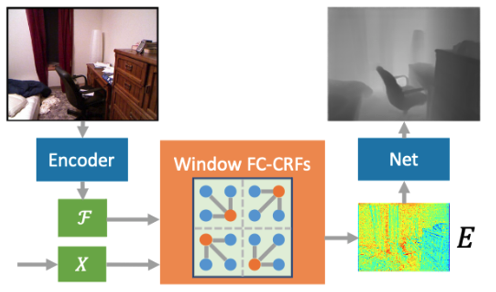
\includegraphics[width=\linewidth]{figures/Monocular_depth/new.png}
    \caption{General structure of NeWCRFs.}
    \label{fig:new}
\end{figure}

\subsubsection{Multiocular Depth Estimation}

\cite{multiview_depthestimation_epipolar, multiview_depthestimation_fusion}

\cite{multiview_depthestimation_RealSense_and_any}

\subsubsection{Depth Completion}

https://paperswithcode.com/sota/depth-completion-on-kitti-depth-completion

\cite{depthcompletion_FusionNet, depthcompletion_NLSPN, depthcompletion_PENet, depthcompletion_SemAttNet}

Made a lot of progress

\fi

\subsubsection{Filling in the Gaps}

If for some reason the added cameras still have blind spots which leave the ground truth incomplete, we have to find a way to recover as much information as possible. Luckily there are algorithms, which make it possible, to extract missing data points.

\subsection{Camera related Experiments}

Performance of multiple cameras can vary from camera to camera. We notice that the usage of multiple cameras has a drastic influence on the performance of the program. Furthermore, if we use multiple cameras, there is a high chance of interference since most cameras use infrared light in the same spectrum [CITE SOMETHING ABOUT INTERFERENCE BETWEEN DEPTH CAMERAS]

To mitigate the interference we conduct some experiments to determine different effects of camera placement on the number of corrupted pixels. We theorise that due to how the cameras work (Scattered-light) the relative translation of the camera might have an influence on the interference.

\subsubsection{Relative Position}

Firstly, we will investigate the relative position of the cameras. We will investigate a close translation in the x axis and the y axis as well as a far translation. The different Camera Positions can be seen in Figure \ref{fig:camera_positions}


\begin{figure}[h]
    \subfloat{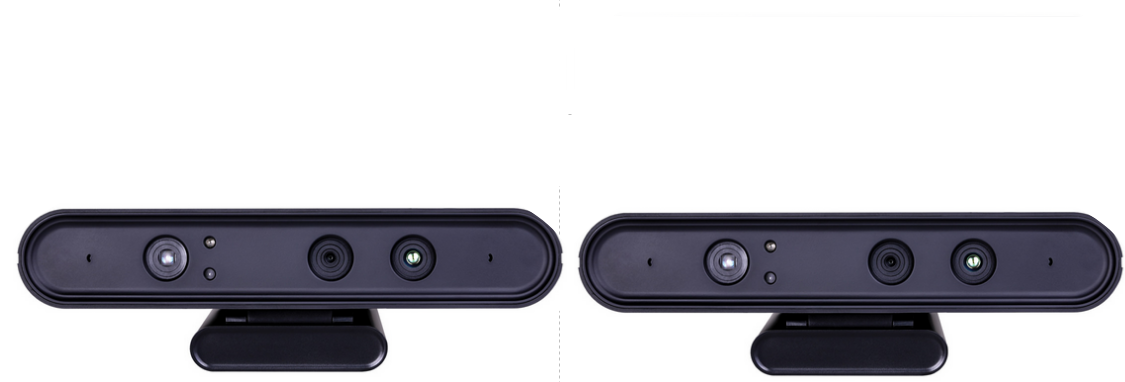
\includegraphics[width=.3\linewidth]{figures/Camera Experiments/x_translation.png}}
    \subfloat{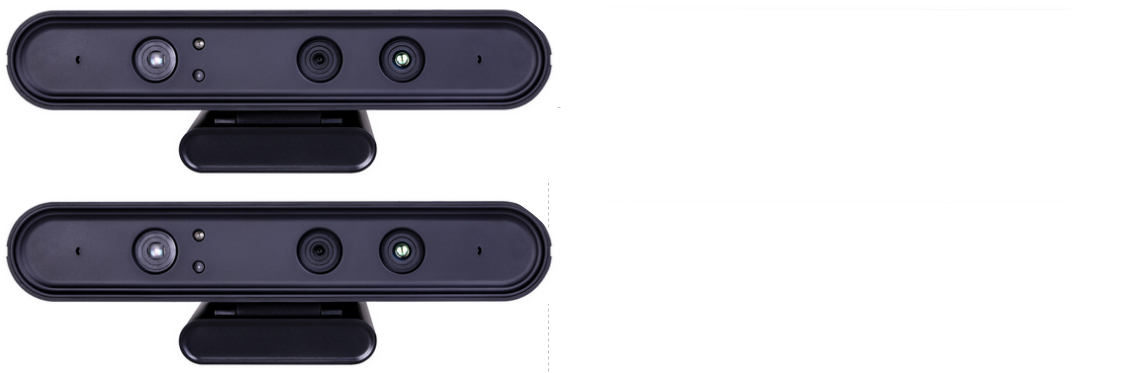
\includegraphics[width=.3\linewidth]{figures/Camera Experiments/y_translation.png}}
    \subfloat{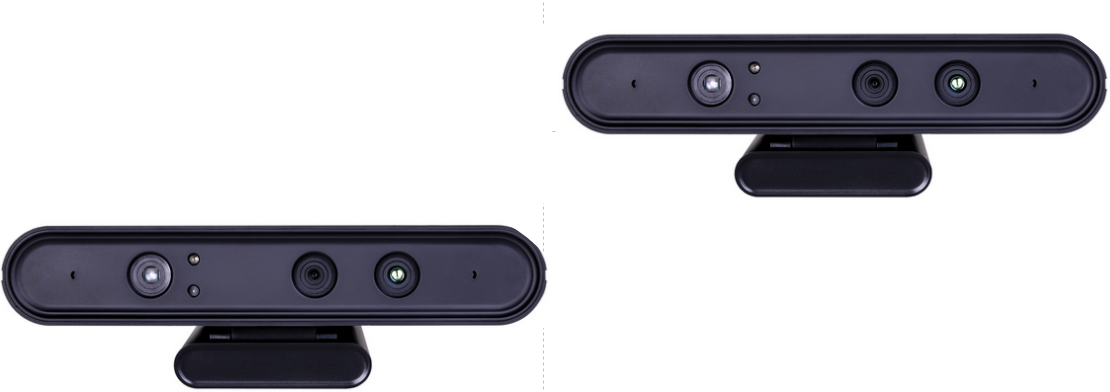
\includegraphics[width=.3\linewidth]{figures/Camera Experiments/x_y_translation.png}} 
    \caption{Different Camera Positions}
    \label{fig:camera_positions}
\end{figure}


Points with a depth value of 0 are invalid depth pixels, which are either not measured by the camera, too close to the camera or too far from the camera. We measure the percentage of invalid depth points for a number of frames.

Firstly we measure the number of invalid pixels for a single camera. For the scene we picked recorded the ceiling, since there are no reflective objects, the distance was just right and the "mounting" of the camera is more simple.

For this setup, we measured an invalid camera pixel rate of $9.18\%$ for a single camera as the average of 1000 consecutively captured frames.

% Please add the following required packages to your document preamble:
% \usepackage{lscape}
\begin{landscape}
\begin{table}[]
\caption{}
\label{tab:different camera positions}
\begin{tabular}{lc|ccc|ccc|ccc}
                        &                       & \multicolumn{3}{c|}{0°}    & \multicolumn{3}{c|}{45°} & \multicolumn{3}{c}{90°} \\
                        & \multicolumn{1}{l|}{} & Mean    & Median  & Std    & Mean    & Median & Std   & Mean   & Median  & Std  \\ \hline
Single Camera           & \multicolumn{1}{l|}{} & 1.48137 & 1       & 0.0157 & -       & -      & -     & -      & -       & -    \\ \hline
Side by side            & Camera 0              & 1.462   & 1       & 0.023  & 1.4544  & 1.4541 & 0.017 &        &         &      \\
                        & Camera 1              & 15.262  & 15      & 0.844  & 14.16   & 14.23  & 0.44  &        &         &      \\ \hline
On top                  & Camera 0              & 1.461   & 1       & 0.0161 &         &        &       &        &         &      \\
                        & Camera 1              & 21.55   & 21      & 1.248  &         &        &       &        &         &      \\ \hline
On top and side by side & Camera 0              & 1.879   & 1.885   & 0.095  &         &        &       &        &         &      \\
                        & Camera 1              & 21.1084 & 21.1025 & 0.524  &         &        &       &        &         &     
\end{tabular}
\end{table}
\end{landscape}

Although promising, on further inspection, the results were refuted, due to the fact that the translation and especially the rotation lead to areas which were not overlapping and therefore not invalidated by overlapping patterns.

This experiment however, shows that one Camera, in this case Camera 0, is less affected than the other. Camera 0, according to the results, does not seem to be affected at all by the secondary camera.

\subsubsection{Using the cameras on different systems}

Another thought that occurs is that the invalid pixels stem from the camera orchestration within the SDK. There are two different levels of test that can be conducted. The first level is the system level. If we run both cameras in different programs using different SDK the orchistration might be different enough to not interfere.

TODOTODO

We ran experiments and this did not work. Whoop de doo.

TODOTODO

The next level is to connect both cameras to different computers. TODO experiments

\subsubsection{Camera Alignment}

When using multiple cameras it is important that the exact relative position is known.